\chapter{Lec 19 - Reinforcement Learning}

\section{Reinforcement Learning}
An \textbf{Agent} operates in an environment $e$, which in response to action $a$ (given by the agent) in the state $s$ returns the next state and a reward $r$ (which can be positive, negative or neutral). The goal of the Agent is to maximize a reward function.\\\\
In many complex domains, reinforcement learning is the only feasible way to train a program to perform at high levels. For example, in game playing, it is very hard for a human to provide accurate and consistent evaluations of large numbers of positions, which would be needed to train an evaluation function directly from examples.  Instead, the program can be told when it has won or lost, and it can use this information to learn an evaluation function that gives reasonably accurate estimates of the  probability of winning from any given position.\\\\
We will assume that the agent does not know how the environment works or what its actions do, and we will allow for probabilistic action outcomes. Thus, the agent faces an unknown Markov decision process. It consists of the set of all the states $S$, the action set $A$, the transition function $\delta$, and the reward function $R$. A Markov decision process relies on the following assumption: the probability of future state $s_{t+1}$ only depends on the current state and action $s_t$, $a_t$,  and doesn’t depend on any of the previous states and actions.\\\\
At each discrete time $t$:
\begin{itemize}
    \item the agent observes state $s_t \in S$;
    \item it chooses action $a_t \in A$ (among the possible actions in state $s_t$);
    \item  it receives immediate reward $r_t$, that can be positive, negative or neutral.
    \item  the state changes to $s_{t+1}$
\end{itemize}
As we said before, we assume that $r_t$ and $s_{t+1}$ only depend on current state and action. Note that $\delta$ and $r$ may be nondeterministic and not necessarily known to agent.\\\\
More formally, the agent's goal is to learn an action policy $\pi: S \rightarrow A$ that maximizes the expected sum of (discounted) rewards obtained if policy $\pi$ is followed:
\[E=\sum_{t=0}^\infty \gamma^t R(s_t)\]
where $\gamma$ is called the \textbf{discount factor}. Note that with discounted rewards, the utility of an infinite sequence is finite. Furthermore, The closer $\gamma$ is to 0, the more the agent will try to optimize the current reward $r_t$. The closer $\gamma$ is to 1, the more the agent will aim to optimize future rewards.

\section{What to Learn}
To begin, consider \textbf{deterministic} environments: for each possible policy $\pi$ the agent might adopt, we can define an evaluation function over states:
\[V^\pi(s) = \sum_{i=0}^\infty \gamma^i r_{t+i}\]
where $r_t, r_{t+1}, ...$ are generated executing policy $\pi$ starting at state $s$. Then the choice of the best actions to play becomes an optimization problem. Indeed, it comes down to finding the optimal policy $\pi^*$ that maximizes the evaluation function:
\[\pi^* = argmax_\pi V^\pi (s)\]
So, how can we find the optimal policy $\pi^*$?\\\\
We might try to have agent learn the evaluation function $V^{\pi^*}$
(which we write as $V^*$).
\begin{equation}
    \pi^* (s) = argmax_a[r(s,a) + \gamma V^*(\delta(s,a))]
\end{equation}
Unfortunately, learning $V^*$ is a useful way to learn the optimal policy only when the agent has perfect knowledge of $\delta$ and $r$. This requires that it be  able to perfectly  predict the immediate result (i.e., the immediate reward and immediate successor) for every possible state-action transition. In many practical problems, it is impossible for the agent or its human programmer to predict in advance the exact outcome of applying an arbitrary action to an  arbitrary state.

\subsection{Q-learning}
Let us define the evaluation function $Q(s, a)$ so that its value is the maximum discounted cumulative reward that can be achieved starting from state $s$ and applying action $a$ as the first action. In other words, the value of $Q$ is the reward received immediately upon executing action $a$ from state $s$, plus the value  (discounted by $\gamma$) of following the optimal policy thereafter.
\[Q(s,a) = r(s,a) + \gamma V^*(\delta(s,a))\]
Then, we can rewrite (1) as:
\[\pi^* (s) = argmax_a Q(s,a)\]
Why is this rewrite  important? Because it shows that if the agent learns the $Q$ function instead of the $V^*$ function, it will be  able to select optimal actions even when it has no knowledge of the functions $r$ and $\delta$.

\subsection{An Algorithm for Learning \textit{Q}}
The key problem  is finding a reliable way to  estimate training  values for $Q$, given  only a sequence of immediate rewards $r$ spread out over time. This can be accomplished through  iterative approximation. To see how,  notice the  close relationship between $Q$ and $V^*$:
\[V^*(s) = max_{a'}Q(s, a')\]
Which allows us to write $Q$ \textbf{recursively} as:
\[
\begin{split}
    Q(s_t, a_t) & = r(s_t, a_t) + \gamma \, V^*(\delta(s_t, a_t))\\
    & = r(s_t, a_t) + \gamma \, max_{a'}Q(s_{t+1}, a')
\end{split}
\]
This recursive definition of $Q$ provides the basis for algorithms that iteratively approximate $Q$.\\\\
Let $\hat{Q}$ denote learner’s current approximation to $Q$. The agent repeatedly observes its current state $s$, chooses some action $a$, executes this action, then observes the resulting reward $r = r(s, a)$ and the new state $s' = \delta(s, a)$. Then, it updates $\hat{Q}$ as follows:
\[\hat{Q}(s,a) = r + \gamma \, max_{a'}\hat{Q}(s', a')\]
The above $Q$ learning algorithm for \textbf{deterministic} Markov decision processes is described more precisely as follows:
\begin{center}
    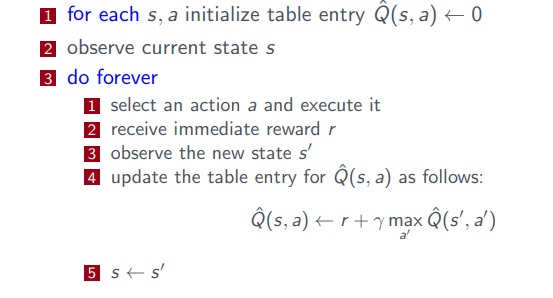
\includegraphics[]{images/Q-learning.png}
\end{center}
Notice the algorithm does not specify how actions are chosen by the agent. One obvious strategy would be for the agent in state $s$ to select the action $a$ that maximizes $\hat{Q}(s, a)$, thereby \textbf{exploiting} its current approximation $\hat{Q}$.  However, with  this strategy the agent runs the risk that it will overcommit to actions  that are found during early training to have high $\hat{Q}$ values, while failing to explore other actions that have even higher values. For this reason, it is common in $Q$ learning to use a probabilistic approach to selecting actions.  Actions with higher $\hat{Q}$ values are assigned higher probabilities, but every action is assigned a nonzero probability. Usually the agent favors \textbf{exploration} during early stages of learning, then gradually shifts toward a strategy of exploitation.
\begin{center}
    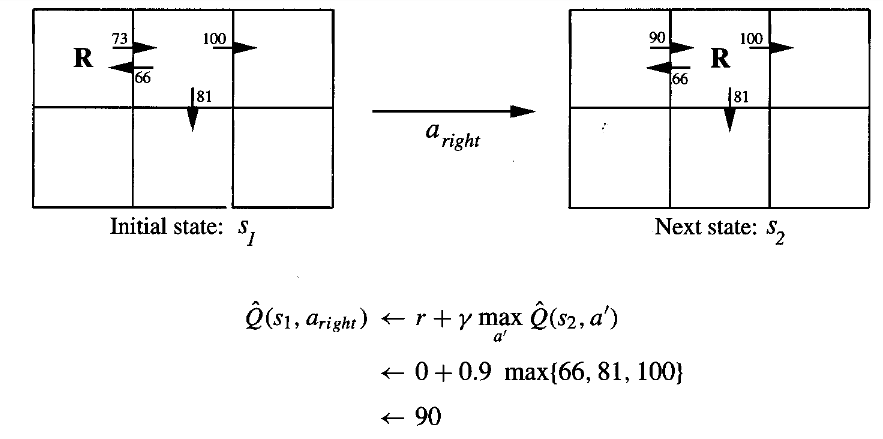
\includegraphics[scale=0.9]{images/Q-learning-ex.png}
\end{center}
Notice if rewards are non-negative, then:
\[(\forall s, a, n) \quad \hat{Q}_{n+1}(s,a) \geq \hat{Q}_n (s,a)\]
where $n$ denotes the $n$-th iteration. A second general property that holds is that through-out the training process every $\hat{Q}$ value will remain in the interval between zero and its true $Q$ value:
\[(\forall s, a, n) \quad 0 \leq \hat{Q}_n (s,a) \leq Q(s,a)\]

\subsection{Convergence}
Will the algorithm above  converge toward a $\hat{Q}$ equal to the true $Q$ function? The answer is yes, under certain conditions. First, we must assume the system is a deterministic MDP. Second, we must assume the immediate reward values are bounded. Third, we assume the agent selects actions in such a fashion that it  visits every possible state-action pair infinitely often.\\\\
The key idea underlying the proof of convergence is that the table entry $\hat{Q}(s,a)$ with the largest error must have its error reduced by a factor of $\gamma$ whenever it is updated.\\\\
Let $\hat{Q}_n$ be the table storing the values for each $(s,a)$ after $n$ updates, and $\Delta_n$ be the maximum error in $\hat{Q}_n$, i.e.
\[\Delta_n = max_{s,a}|\,\hat{Q}_n(s,a) - Q(s,a)\,|\]
For any table entry $\hat{Q}_n(s, a)$ updated on iteration $n + 1$, the error in the revised estimate $\hat{Q}_{n+1}(s, a)$ is:
\begin{center}
    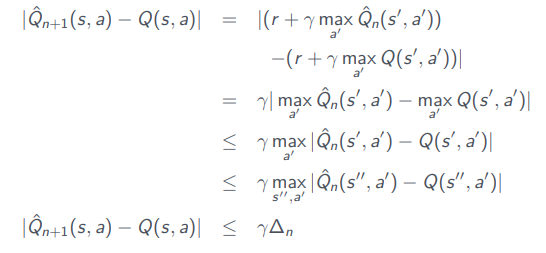
\includegraphics[]{images/Q-learning-conv-proof.png}
\end{center}
Note we used general fact that:
\[|\,max_a f_1(a) - max_a f_2(a)\,| \leq max_a|\,f_1(a) - f_2(a)\,|\]

\subsection{Nondeterministic Case}
Above we considered $Q$ learning in deterministic environments. Here we consider the nondeterministic case, in which the reward function $r(s, a)$ and action transition function $\delta(s, a)$ may have probabilistic outcomes.\\\\
In this section we extend the $Q$ learning  algorithm for the deterministic case to handle nondeterministic MDPs. In the nondeterministic case we must first restate the objective of the learner to take into account the fact that outcomes of actions are no longer deterministic. The obvious generalization is to redefine the value $V^\pi$ of a policy $\pi$ to be the expected value (over these nondeterministic outcomes) of the discounted cumulative reward  received by applying this policy.
\[V^\pi(s_t) = E\left[\sum_{i=0}^\infty \gamma^i r_{t+i} \right]\]
As before, we define the optimal policy $\pi^*$ to be the policy $\pi$ that maximizes $V^\pi(s)$ for all states $s$. Next  we generalize our earlier definition of $Q$ by taking its expected value.
\[Q(s,a) = E[r(s,a) + \gamma V^*(\delta(s,a))]\]
To learn, alter training rule to:
\begin{equation}
    \hat{Q}_n(s,a) \leftarrow (1 - \alpha_n)\hat{Q}_{n-1}(s,a) + \alpha_n [r + \gamma \, max_{a'}\hat{Q}_{n-1}(s', a')]
\end{equation}
where
\[\alpha_n = \frac{1}{1 + visits_n(s,a)}\]
where $visits_n(s,a)$  is the  total number of times this state-action pair  has been visited up to and including the $n$-th iteration. The key idea in this revised rule is that revisions to $\hat{Q}$ are made more gradually than in  the deterministic case. Notice if we were to set $\alpha_n$ to 1 we would have exactly the training rule for the deterministic case. Under specific conditions, can still prove convergence of $\hat{Q}$ to $Q$.

\subsection{Temporal Difference Learning (TD-lambda)}
The $Q$ learning algorithm learns by iteratively \textbf{reducing the discrepancy} between $Q$ value estimates for adjacent state. In this sense, $Q$ learning is a special case of a general class of temporal diflerence algorithms that learn by reducing discrepancies between estimates made by the agent at different times.\\\\
Whereas the training rule of Equation (2) reduces the difference between the estimated $\hat{Q}$ values of a state and its immediate successor, we could just as well design an algorithm that reduces discrepancies between this state and  more distant descendants or ancestors.
\[Q^{(2)}(s_t, a_t) = r_t + \gamma r_{t+1} + \gamma^2 max_a \hat{Q}(s_{t+2}, a)\]
or, in general, for $n$ steps
\[Q^{(n)}(s_t, a_t) = r_t + \gamma r_{t+1} + ... + \gamma^{n-1}r_{t+n-1} + \gamma^n max_a \hat{Q}(s_{t+n}, a)\]
Sutton (1988) introduces a general method for blending  these alternative training estimates, called $TD(\lambda)$. The idea  is to use a constant $0 \leq \lambda \leq 1$ to combine the estimates obtained from various lookahead distances in the following fashion:
\[Q^\lambda (s_t, a_t) = (1-\lambda)\left[ Q^{(1)}(s_t, a_t) + \lambda Q^{(2)}(s_t, a_t) + \lambda^2 Q^{(3)}(s_t, a_t) + ...\right]\]
Note if we choose $\lambda = 0$ we have our original training estimate $Q^{(1)}$, which considers only one-step discrepancies in the $\hat{Q}$ estimates. As $\lambda$ is increased, the algorithm places increasing emphasis on discrepancies based on more distant lookaheads.\\\\
Many improvements/extensions are possible, for example, we can replace $\hat{Q}$ table with a (deep) neural net!

